\documentclass{article}

\usepackage{algorithm,algpseudocode}
\usepackage[margin=1in]{geometry}
\usepackage{enumerate}
\usepackage{multicol}
\usepackage{graphicx}
\DeclareGraphicsExtensions{.pdf,.PDF,.png,.PNG}
\graphicspath{{figs/}}

\usepackage{amsfonts,amsmath}
\def\R{{\mathbb R}}
\def\N{{\mathbb N}}

\title{In-Class Exercise 10}
\author{CSCI 432}
\date{28 October 2019}

\begin{document}
\maketitle

\noindent
Group Number:\\
Group members present today:

\section*{Linear Programming}

\begin{multicols}{2}

\begin{enumerate}
    \item On this graph paper, draw the following lines:
        \begin{align}
            4x_1 - x_2 &= 8\\
            2x_1 + x_2 &= 10\\
            5x_1 -2x_2 &= -2 \\
            x_1 &= 0\\
            x_2 &= 0
        \end{align}
        HINT: use the bottom
        left corner as the point~$(0,0)$
    \item Shade in the feasible space of points $(x_1,x_2)\in \R^2)$ that
        satisfy the following~inequalities:
        \begin{align}
            4x_1 - x_2 &\leq 8\\
            2x_1 + x_2 &\leq 10\\
            5x_1 -2x_2 &\geq -2 \\
            x_1 &\geq 0\\
            x_2 &\geq 0
        \end{align}
    \item As dotted lines, draw the lines where $x_1+x_2=0$, $x_1+x_2=2$, and
        $x_1+x_2=2$.  What do you notice about these lines?
        \vspace{.75in}
    \item Suppose we want to maximize $x_1+x_2$ subject to the constraints
        above.  It turns out that the answer always lies on a vertex of the
        space you just shaded!  Compute $f(x_1,x_2)=x_1+x_2$ for each of the
        vertices. Which point attains the maximum value?
        \vspace{.75in}
    \item Write this linear program in standard form.\\
        \vspace{2in}
    \item What happens if I change the last constraint to~$x_1 \leq 0$?
\end{enumerate}

\end{multicols}

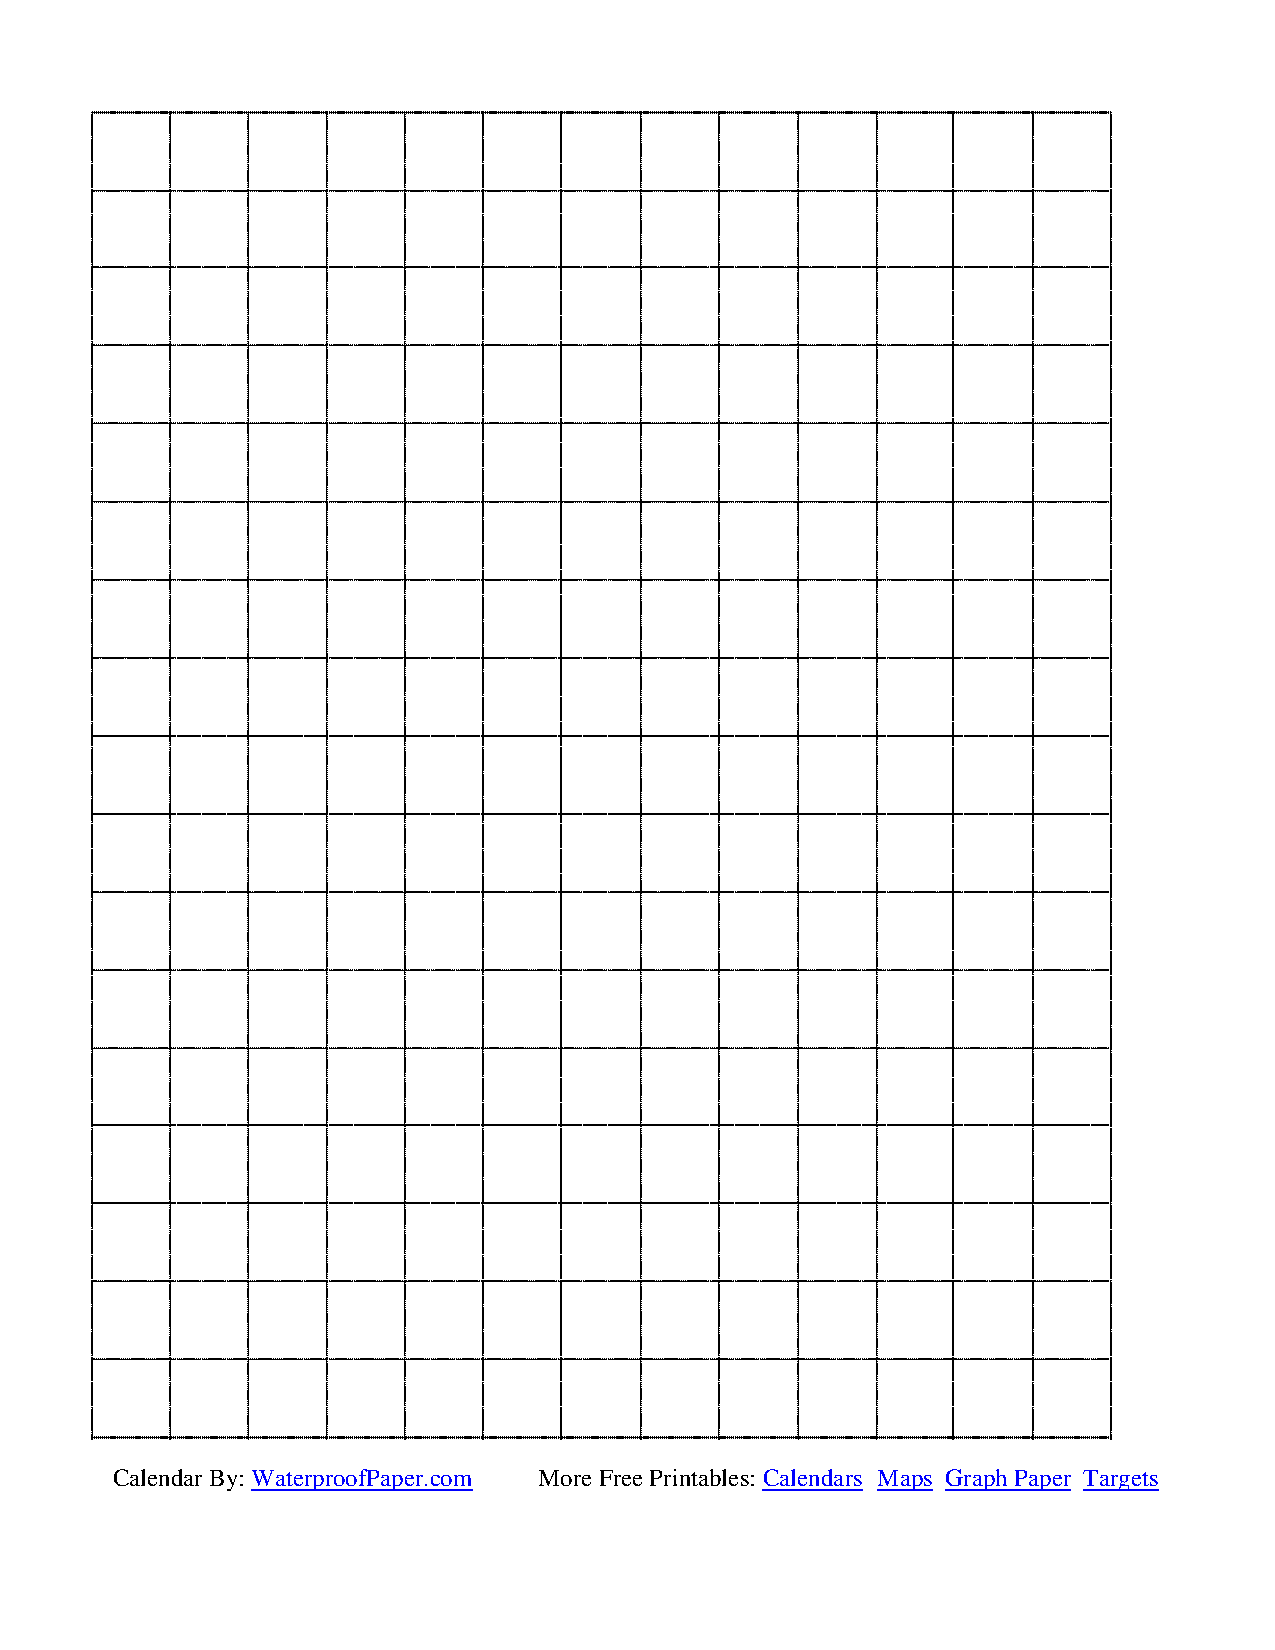
\includegraphics[width=\textwidth]{graph-paper}

\end{document}
